\uuid{6990}
\auteur{blanc-centi}
\datecreate{2015-07-04}
\isIndication{true}
\isCorrection{true}
\chapitre{Courbes planes}
\sousChapitre{Coordonnées polaires}

\contenu{
\texte{
On considère les courbes $\mathcal{C}_1$ et $\mathcal{C}_2$ {\it (des limaçons de Pascal)} 
respectivement données en polaires par 
$$r_1(\theta)=1+\cos\theta\quad\quad r_2(\theta)=3+\cos\theta$$
Pour $i=1,2$, on note $N_i(\theta)$ la droite orthogonale au point $M_i(\theta)\in\mathcal{C}_i$. 
Vérifier que pour tout $\theta\not\equiv 0\ [2\pi]$, les droites $N_1(\theta)$ et $N_2(\theta)$ sont sécantes, en un point $P(\theta)$. Déterminer le lieu du point $P$ quand $\theta$ varie.
}
\indication{Utiliser le repère de Frenet $(\vec{u}_\theta,\vec{v}_\theta)$.}
\reponse{
Les deux équations sont $2\pi$-périodiques en $\theta$, soit donc $\theta\in[0;2\pi[$, cherchons pour chaque courbe le vecteur tangent au point $M_i(\theta)$. Déjà, $\mathcal{C}_2$ ne passe pas par le p\^ole mais $\mathcal{C}_1$ oui, pour $\theta=\pi$: elle a donc en $M_1(\pi)$ une tangente horizontale (dirigée par le vecteur $\vec{u}_\pi$) et $N_1(\pi)$ est l'axe $(Oy)$. Dans tous les autres cas, la tangente à $\mathcal{C}_i$ au point $M_i(\theta)$ est dirigée par le vecteur
$$\overrightarrow{\frac{\dd OM_i}{\dd \theta}}(\theta)=r'(\theta)\vec{u}_\theta+r(\theta)\vec{v}_\theta=-\sin\theta\,\vec{u}_\theta+(a_i+\cos\theta)\vec{v}_\theta$$
où $a_1=1,a_2=3$. Le vecteur directeur de $N_i(\theta)$ est donc
$$\vec{n_i}(\theta):=(a_i+\cos\theta)\vec{u}_\theta+\sin\theta\,\vec{v}_\theta$$ 
et 
$M\in N_i(\theta)\Longleftrightarrow \exists t\in\R\ |\ \overrightarrow{OM}=\overrightarrow{OM_i(\theta)}+t\cdot\vec{n_i}(\theta)$.
Finalement, 
$$\forall \theta\not=\pi,\ N_i(\theta)
=\big\{(1+t)(a_i+\cos\theta)\vec{u}_\theta+t\sin\theta\,\vec{v}_\theta\ |\ t\in\R\big\}$$
et le résultat s'étend au cas $\theta=\pi$ pour $i=2$.
\begin{itemize}
\item Si $\theta=\pi$, $N_1(\pi)=(Oy)$ et $N_2(\pi)=\{2(1+t)\vec{u}_\pi\ |\ t\in\R\}=(Ox)$, ces deux droites s'intersectent en $O$.
\item Si $\theta\not=\pi$, $N_1(\theta)$ et $N_2(\theta)$ sont sécantes si et seulement si les vecteurs $\vec{n_1}(\theta)$ et $\vec{n_2}(\theta)$ ne sont pas colinéaires, c'est-à-dire si et seulement si $\begin{array}{|cc|}1+\cos\theta&3+\cos\theta\\ \sin\theta&\sin\theta\end{array}\not=0$ \textsl{i.e.} $\sin\theta\not=0$. Ainsi, pour $\theta\not=0$, les droites $N_1(\theta)$ et $N_2(\theta)$ sont sécantes en un point $P(\theta)$, que l'on peut déterminer: 
\begin{eqnarray*}
\lefteqn{(1+t_1)(1+\cos\theta)\vec{u}_\theta+t_1\sin\theta\,\vec{v}_\theta=(1+t_2)(3+\cos\theta)\vec{u}_\theta+t_2\sin\theta\,\vec{v}_\theta}\\
&\Longleftrightarrow& \begin{cases}(1+t_1)(1+\cos\theta)=(1+t_2)(3+\cos\theta)\cr t_1\sin\theta=t_2\sin\theta\end{cases}\\
&\Longleftrightarrow& \begin{cases}t_1=-1\cr t_1=t_2\end{cases}
\end{eqnarray*}
puisqu'ici $\sin\theta\not=0$. 
On obtient alors $\overrightarrow{OP(\theta)}=-\sin\theta\,\vec{v}_\theta$. 
\end{itemize}

La formule donnant $P(\theta)$ pour $\theta\not=\pi$ est en fait encore valable en $\theta=\pi$ puisqu'on retrouve dans ce cas $P(\pi)=O$. En coordonnées cartésiennes, on a donc
$$\forall\theta\in]0;2\pi[,\ P(\theta)=(\sin^2\theta, -\sin\theta\cos\theta)$$
Remarquons que 
\begin{eqnarray*}
(\sin^2\theta, -\sin\theta\cos\theta)&=&\left(\frac{1-\cos(2\theta)}{2},-\frac{1}{2}\sin(2\theta)\right)\\
 &=&\left(\frac{1}{2},0\right)-\frac{1}{2}\big(\cos(2\theta),\sin(2\theta)\big)
\end{eqnarray*}
Lorsque $\theta$ décrit $]0;2\pi[$, $2\theta$ décrit $]0;4\pi[$ et 
$\big(\cos(2\theta),\sin(2\theta)\big)$ décrit (deux fois, sauf en $(1,0)$ où l'on ne passe 
qu'une fois) le cercle unité. Par conséquent $\{P(\theta)\ |\ \theta\in]0;2\pi[\}$ 
est le cercle de centre $(\frac{1}{2},0)$ et de rayon $\frac{1}{2}$.

\begin{center}
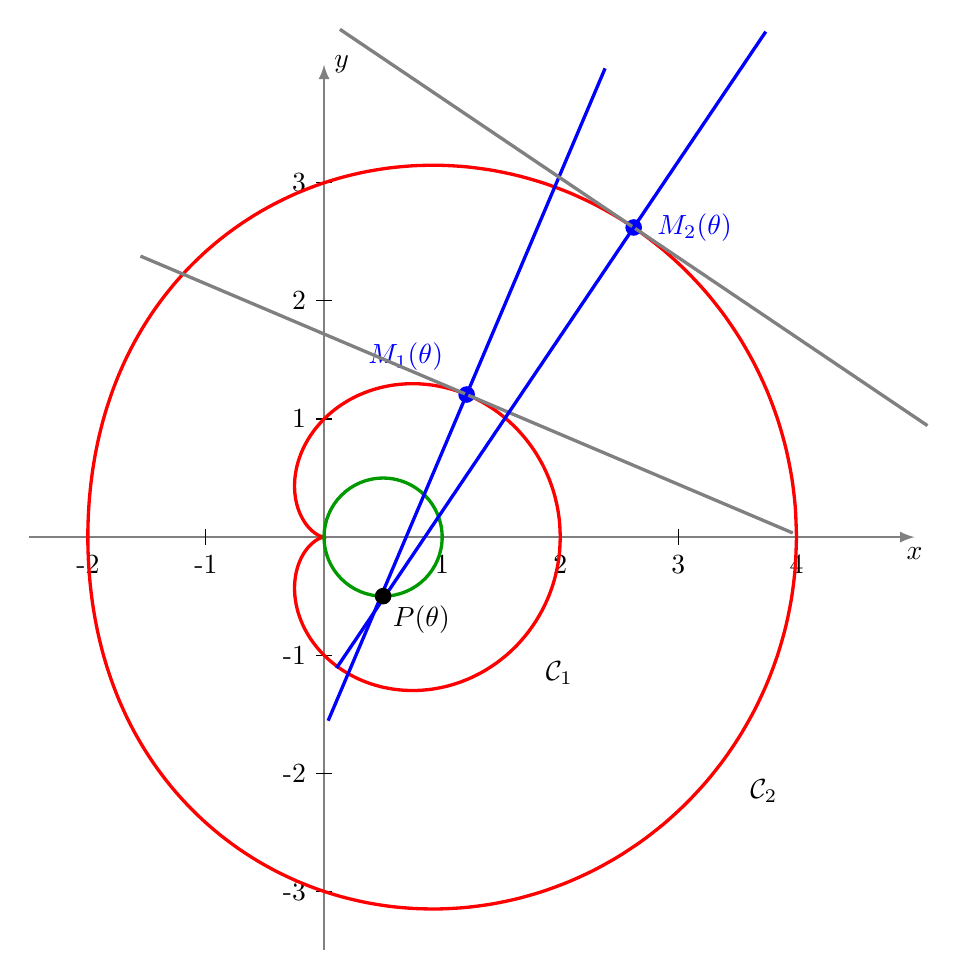
\begin{tikzpicture}[scale=1.5]

% Axes
     \draw[->,>=latex,thick, gray] (-2.5,0)--(5,0) node[below,black] {$x$};
     \draw[->,>=latex,thick, gray] (0,-3.5)--(0,4) node[right,black] {$y$};  

 % Ticks
        \foreach \x in {1,...,4}
                \draw (\x,2pt) -- (\x,-2pt)
                        node[anchor=north] {\x};
        \foreach \x in {-1,-2}
                \draw (\x,2pt) -- (\x,-2pt)
                        node[anchor=north] {\x};
        \foreach \x in {1,2,3}
                \draw (2pt,\x) -- (-2pt,\x)
                        node[anchor=east] {\x};
        \foreach \x in {-1,-2,-3}
                \draw (2pt,\x) -- (-2pt,\x)
                        node[anchor=east] {\x};



% Courbe

\draw [very thick, color=red, domain=0:2*pi, samples=100, smooth]
  plot (xy polar cs:angle=\x r, radius={1+cos(\x r)});


\draw [very thick, color=red, domain=0:2*pi, samples=100, smooth]
  plot (xy polar cs:angle=\x r, radius={3+cos(\x r)});

\draw [very thick, color=green!60!black] (0.5,0) circle (0.5cm);


  \coordinate (M1) at (45:1.707);
  \fill[blue] (M1) circle (2pt)  node[above left=5pt]{$M_1(\theta)$}; 
  \draw[very thick, gray] (M1)--+(-23:3)--+(-23:-3);
  \draw[very thick, blue] (M1)--+(90-23:3)--+(90-23:-3);

  \coordinate (M2) at (45:3.707);
  \fill[blue] (M2) circle (2pt)  node[right=5pt]{$M_2(\theta)$}; 
  \draw[very thick, gray] (M2)--+(-34:3)--+(-34:-3);
  \draw[very thick, blue] (M2)--+(90-34:2)--+(90-34:-4.5);

   \fill [color=black]  (0.5,-0.5) circle (2pt) node[below right] {$P(\theta)$};

  \node at (-30:2.3) {$\mathcal{C}_1$};
  \node at (-30:4.3) {$\mathcal{C}_2$};
\end{tikzpicture}  
\end{center}
}
}
